%	p0/.style={circle,fill=yellow,thick},p1/.style={rectangle,fill=green,thick}
\documentclass{article}
\usepackage{tikz}
\usetikzlibrary{automata,calc}
\usetikzlibrary{arrows}

\begin{document}
	
	\begin{center}
		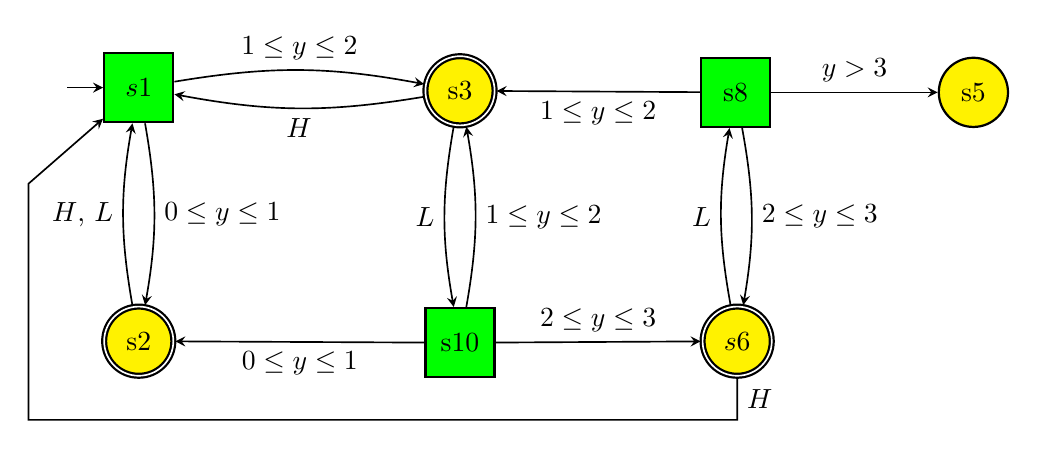
\begin{tikzpicture}[
		auto,
		initial text=,
		semithick,
		>=stealth,
		,
		p0/.style={circle,fill=yellow,thick},p1/.style={rectangle,fill=green,thick}
		]
		\node[state,initial,p1](s1) at (6.44,2.24){$s1$};
		\node[state,accepting,p0](s2) at (6.44,-0.98){s2};
		\node[state,accepting,p0](s3) at (10.52,2.2){s3};
		\node[state,p0](s5) at (17.04,2.18){s5};
		\node[state,accepting,p0](s6) at (14.04,-0.98){$s6$};
		\node[state,p1](s8) at (14.02,2.18){s8};
		\node[state,p1](s10) at (10.52,-1.0){s10};
		\path[->]
		(s1) edge [bend left=10] node {$0 \leq y \leq 1$} (s2)
		(s1) edge [bend left=10] node {$1 \leq y \leq 2$} (s3)
		(s2) edge [bend left=10] node {$H$,\ $L$} (s1)
		(s3) edge [bend left=10] node {$H$} (s1)
		(s3) edge [bend right=10] node [left] {$L$} (s10)
		(s6) edge [bend left=10] node {$L$} (s8)
		(s8) edge [] node {$1 \leq y \leq 2$} (s3)
		(s8) edge [] node {$y > 3$} (s5)
		(s8) edge [bend left=10] node {$2 \leq y \leq 3$} (s6)
		(s10) edge [] node {$0 \leq y \leq 1$} (s2)
		(s10) edge [bend right=10] node [right] {$1 \leq y \leq 2$} (s3)
		(s10) edge [] node {$2 \leq y \leq 3$} (s6)
		;
		
		\path[->,draw] (s6) --  node {$H$} ++(0,-1) -- ++(-9,0) -- ++(0,3) -- (s1);
		
		
		\end{tikzpicture}
	\end{center}



	\begin{center}
		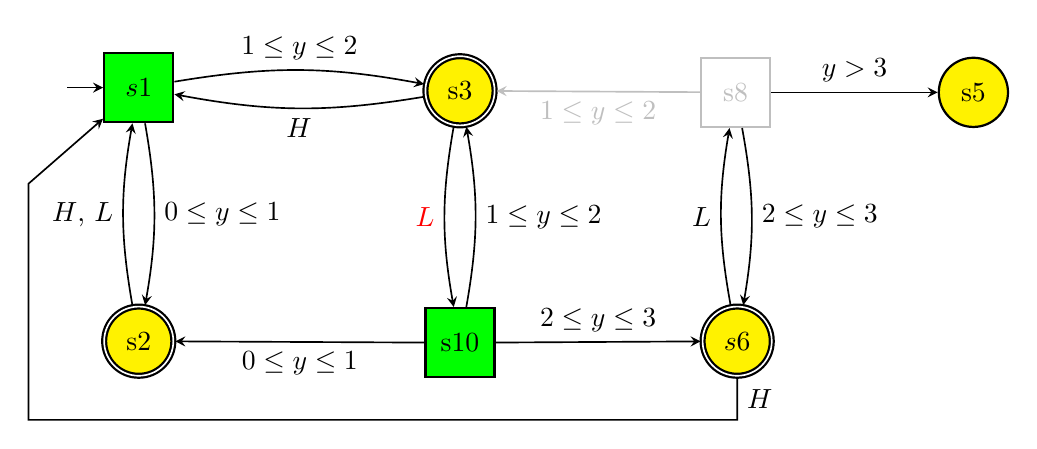
\begin{tikzpicture}[
		auto,
		initial text=,
		semithick,
		>=stealth,
		,
		p0/.style={circle,fill=yellow,thick},p1/.style={rectangle,fill=green,thick}
		]
		\node[state,initial,p1](s1) at (6.44,2.24){$s1$};
		\node[state,accepting,p0](s2) at (6.44,-0.98){s2};
		\node[state,accepting,p0](s3) at (10.52,2.2){s3};
		\node[state,p0](s5) at (17.04,2.18){s5};
		\node[state,accepting,p0](s6) at (14.04,-0.98){$s6$};
		\node[state,p1,fill=white, draw=lightgray,text=lightgray](s8) at (14.02,2.18){s8};
		\node[state,p1](s10) at (10.52,-1.0){s10};
		\path[->]
		(s1) edge [bend left=10] node {$0 \leq y \leq 1$} (s2)
		(s1) edge [bend left=10] node {$1 \leq y \leq 2$} (s3)
		(s2) edge [bend left=10] node {$H$,\ $L$} (s1)
		(s3) edge [bend left=10] node {$H$} (s1)
		(s3) edge [bend right=10,text=red] node [left] {$L$} (s10)
		(s6) edge [bend left=10] node {$L$} (s8)
		(s8) edge [draw=lightgray, text=lightgray] node {$1 \leq y \leq 2$} (s3)
		(s8) edge [] node {$y > 3$} (s5)
		(s8) edge [bend left=10] node {$2 \leq y \leq 3$} (s6)
		(s10) edge [] node {$0 \leq y \leq 1$} (s2)
		(s10) edge [bend right=10] node [right] {$1 \leq y \leq 2$} (s3)
		(s10) edge [] node {$2 \leq y \leq 3$} (s6)
		;
		
		\path[->,draw] (s6) --  node {$H$} ++(0,-1) -- ++(-9,0) -- ++(0,3) -- (s1);
		
		
		\end{tikzpicture}
	\end{center}
\end{document}
